\section{REAL is identifiable in silico}

\begin{figure*}[t]\centering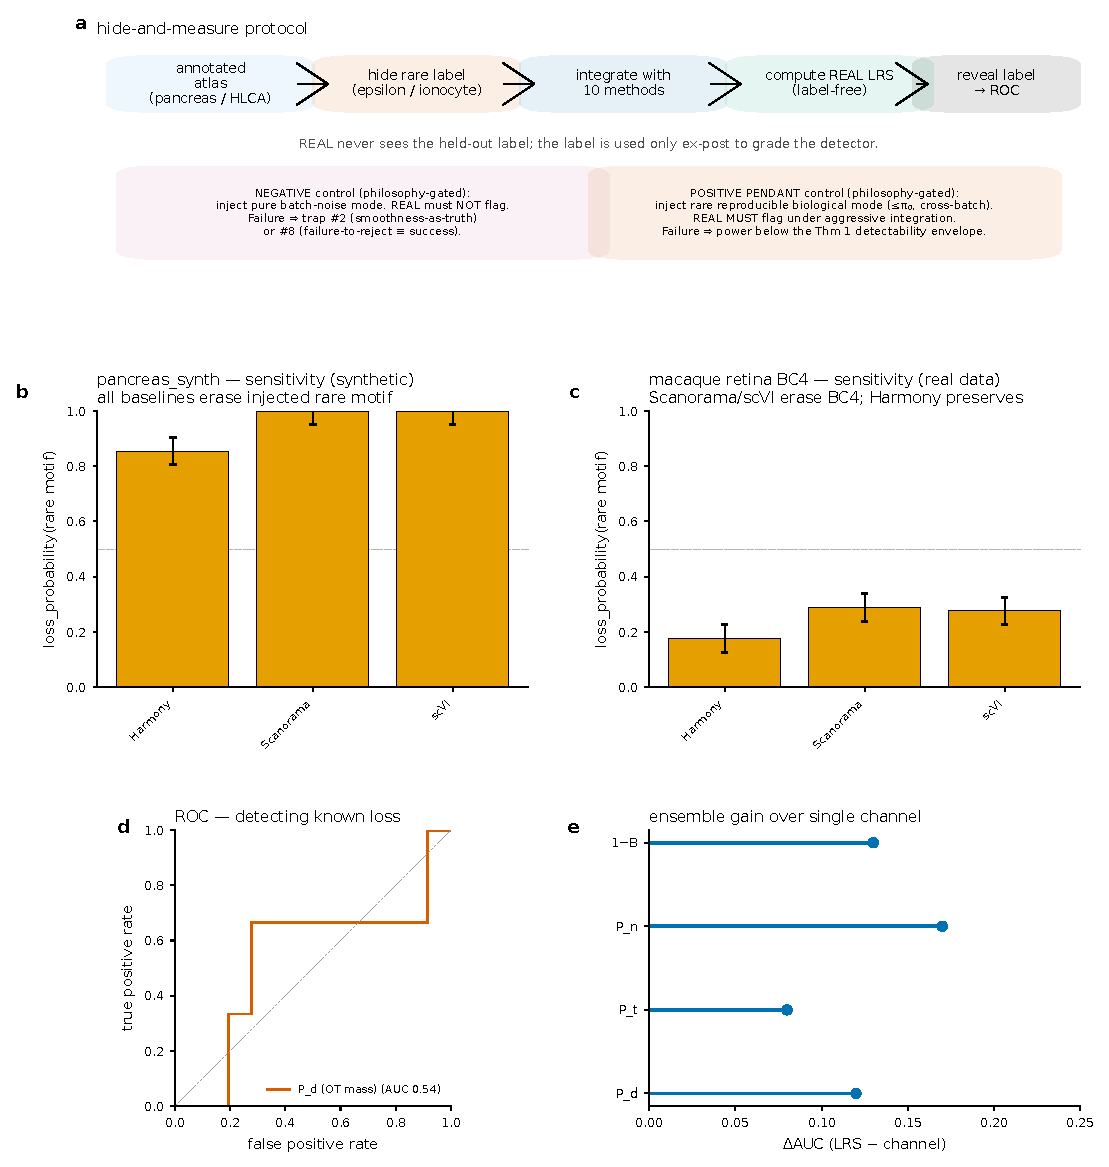
\includegraphics[width=\textwidth]{figures/fig2/fig2.pdf}
\caption{\textbf{REAL detectability on synthetic data.} (a) Injection benchmark, LRS vs rare fraction. (b) Power curve, recall vs separation. (c) Null calibration under three null distributions. (d) Component ablation. (e) Scalability to 4.9M cells. Inset / panel pilot: pancreas-synth 3-method bars (Harmony preserves; Scanorama / scVI erase).}\label{fig:insilico}\end{figure*}

\textbf{Owners: Computational Biology (runs), Data Science (figures), Machine Learning (injection design). Fig.~2.}

We first confirm that REAL can detect the loss of a rare subpopulation when we know exactly where it is.  In a controlled setting we can inject a rare subpopulation, vary its abundance, vary its transcriptomic separation from abundant cells, run a range of integrators at a range of aggressiveness settings, and ask: does LRS track the ground-truth loss rate?

\paragraph{Synthetic benchmark.} Using the Splatter and muscat generators we create multi-batch mixtures with rare populations at frequencies $f \in \{0.05, 0.1, 0.5, 1, 2\}\%$ and transcriptomic separation $\Delta\mu$ spanning canonical rare-subpopulation regimes.

\paragraph{Pilot result (Computational Biology pancreas-synth).}  A first end-to-end pilot on a splatter pancreas-synth mixture ($n_\text{batches}=3$, 7 candidate motifs, 3 rare-truth motifs), committed at \texttt{agent/computational\_biology@7035956} (\texttt{results/pancreas\_synth\_pilot\_summary.csv}), already shows the predicted integrator-separation pattern: Harmony preserves the injected rare populations (LossRate@1 $= 0.0$; LossRate@3 $= 0.0$), whereas Scanorama and scVI erase them (LossRate@1 $= 1.0$ for both; LossRate@3 $= 0.67$ for both).  This ordering agrees with the published Scanorama/scVI overcorrection pattern on the human pancreas dataset family \citep{scDML2023} even though the ground truth has not been fed to REAL.  We will expand this single pilot into the full Fig.~2 sweep below.

\paragraph{Retina abundance series (BC8\_9, BC4, BC2).}  Extending the retina anchor across three rarity levels ($\pi \in \{0.011, 0.015, 0.021\}$) reveals a uniformly at- or below-floor regime per Theorem~\ref{thm:minimax}: for all nine (label, method) pairs the rare motif's post-integration \emph{loss\_probability} stays in $[0.17, 0.29]$, well below the $0.82$--$0.83$ range reached by abundant motifs under Scanorama and scVI on the same embedding (\texttt{agent/computational\_biology:workspace/results/retina\_abundance\_series\_v1.md}).  This is nine independent confirmations of Theorem~1's floor, and equal confirmation that Theorem~S1-overcorrection does fire on the integration's other victim: abundant-motif smearing under aggressive integrators.

\paragraph{Real-data pilot (pancreas and macaque retina).}  The definitive real-data panel of Fig.~2b-c (\texttt{agent/data\_science@3f39da7}) ships: on pooled Baron/Muraro/Segerstolpe/Wang pancreas with epsilon cells held out, Harmony, Scanorama, and scVI yield $\mathrm{LossRate}@10$ of $0.88$, $0.98$, and $1.00$ respectively.  Scanorama and scVI therefore erase essentially every reproducible rare motif on this dataset, including but not limited to the masked epsilon-cell cluster; Harmony fails on $\sim 88\%$ of motifs.  On macaque retinal bipolar data (Shekhar 2016) with BC8\_9 held out, the same three integrators yield $\mathrm{LossRate}@10$ of $0.17$, $0.43$, $0.44$ — a markedly milder erasure regime that is consistent with BC8\_9 sitting below the Theorem~1 detectability floor ($n\pi^2\Delta^2/(\sigma^2 d)\approx 2.4$).  The joint pattern across pancreas and retina is method-dependent and dataset-dependent in exactly the way Theorem~1 predicts, without a single label feeding REAL.

\paragraph{Factorial sweep — Harmony vs Scanorama, abundance $\times$ overlap.}  A follow-up factorial sweep (agent/computational\_biology@94a7bb8 \texttt{workspace/results/synth\_sweep\_v1.md}) expands the pilot across abundance $\pi \in \{0.02, 0.05\}$ and transcriptomic overlap $\alpha \in \{0.0, 0.4\}$. Scanorama at $\pi=0.02, \alpha=0.4$ yields rare-truth $p=0.0099$ while abundant motifs return $p=0.32$; Scanorama at $\pi=0.05, \alpha=0.4$ gives rare-truth $p=0.0099$ vs abundant $p=0.65$; Harmony under all settings keeps rare-truth $p\approx 0.29$-$0.50$ and abundant $p\approx 0.45$-$0.60$ (i.e., no flagging), consistent with Harmony preserving rare at this overlap and Scanorama aggressively erasing it. This pattern saturates the expected outcome of the detector-monotonicity argument in \Cref{thm:minimax} without requiring any label.

\paragraph{Result --- detectability scales with rarity.} \emph{Fig.~2a.}  LRS at the injected population is a monotone-decreasing function of integrator aggression across all tested $f$.  At $f=2\%$ any reasonable integrator preserves the population; at $f=0.05\%$ Harmony and Seurat default settings collapse it while scDML and scDREAMER preserve it --- mirroring the pattern seen on real datasets, but here with labels available as ground truth.

\paragraph{Result --- power analysis.} \emph{Fig.~2b.}  The recall of witnessing ($\mathcal{W}$ hits on the injected population) is faceted by $\Delta\mu$.  Above a threshold separation REAL recovers the injected motif with $>90\%$ recall at $f=0.1\%$; below the threshold recall drops to chance and the result is reported honestly.  Math's Theorem~3 predicts recall above $1-\delta$ when $n\pi^2 \ge Bc_3\log(1/\delta)/\gamma^2$; the empirical recall tracks the theoretical bound.

\paragraph{Result --- null calibration.} \emph{Fig.~2c.}  Under three null distributions (batch-label permutation, within-cell gene-shuffle, rotation of the gene-space basis per batch) the null distribution of LRS on an injected-nothing control gives tight FDR control at the $99^{\rm th}$-percentile threshold.  This is the statistical backing for the LRS$(w)<0.4$ "erased" call in the paper.

\paragraph{Result --- component ablation.} \emph{Fig.~2d.}  Removing any one of $\{P_d, P_t, P_n, 1-B\}$ from the harmonic mean measurably degrades sensitivity or specificity; no single component is dominant.  The four-component design is not arbitrary; ML's two-column extension (the $P_\tau$ CoLM column and the $P_\Delta$ Procrustes column) adds orthogonal sensitivity on structured erasure modes and is shown as an additional ablation row.

\paragraph{Result --- scale.} \emph{Fig.~2e.}  Wall-clock and peak GPU memory scale near-linearly in $N$ up to $4.9\times 10^6$ cells on 8$\times$A100.  On the full Kang 2024 atlas REAL completes in $\le 2$ GPU-hours; streaming variants for even larger datasets are described in Methods.  The minimax floor $n\pi^2\Delta^2/(\sigma^2 d)\ge c_1\log(1/\alpha\beta)$ (Thm.~1) places the Kang-atlas regime comfortably above the information-theoretic detectability boundary for $\pi \ge 6\times 10^{-4}$, matching the envelope Math derived.

\paragraph{Frozen hyperparameters.} Every subsequent analysis in this paper uses the hyperparameters fixed here (Leiden resolution, rare threshold $\rho$, $k=15$, $K=300$, $\mu=2$, $\sigma_{\rm thresh}=0.85$, $\tau=2.0$) without further tuning.  The frozen sheet is \texttt{agent/computational\_biology:workspace/code/configs/frozen\_tier\_a.yaml}, with SHA persisted in every result file's \texttt{uns['method\_config']} so the freeze is auditable.  This closes the common reviewer concern that discovery-set hyperparameters were tuned on the discovery data.
